\documentclass[preprint,12pt,authoryear]{elsarticle}
%\documentclass[final,1p,times,twocolumn,authoryear]{elsarticle}
\usepackage{lineno,hyperref}
\modulolinenumbers[5]

\journal{Journal of \LaTeX\ Templates}

%%%%%%%%%%%%%%%%%%%%%%%
%% Elsevier bibliography styles
%%%%%%%%%%%%%%%%%%%%%%%
%% To change the style, put a % in front of the second line of the current style and
%% remove the % from the second line of the style you would like to use.
%%%%%%%%%%%%%%%%%%%%%%%

%% Numbered
%\bibliographystyle{model1-num-names}

%% Numbered without titles
%\bibliographystyle{model1a-num-names}

%% Harvard
\bibliographystyle{model2-names.bst}\biboptions{authoryear}

%% Vancouver numbered
%\usepackage{numcompress}\bibliographystyle{model3-num-names}

%% Vancouver name/year
%\usepackage{numcompress}\bibliographystyle{model4-names}\biboptions{authoryear}

%% APA style
%\bibliographystyle{model5-names}\biboptions{authoryear}

%% AMA style
%\usepackage{numcompress}\bibliographystyle{model6-num-names}

%% `Elsevier LaTeX' style
%\bibliographystyle{elsarticle-harv}
%%%%%%%%%%%%%%%%%%%%%%%

\begin{document}

\begin{frontmatter}

\title{Joint analysis of geological map units and topography to support soil survey - lessons from a case study in South Tyrol OR From geological to soil parent material maps - a random forest-supported  analysis of geological map units and topography in South Tyrol}


%% Group authors per affiliation:

\author[mymainadress]{Fabian E. Gruber\corref{mycorrespondingauthor}}
\cortext[mycorrespondingauthor]{Corresponding author}
\ead{Fabian.Gruber@uibk.ac.at}
\author[mymainadress]{Jasmin Baruck}
\author[mymainadress]{Clemens Geitner}



\address[mymainadress]{Institute of Geography, University of Innsbruck, Innrain 52f, 6020 Innsbruck, Austria}

\begin{abstract}

\end{abstract}

\begin{keyword}

\end{keyword}

\end{frontmatter}

\linenumbers

\section{Introduction}
\paragraph{general introduction}
Geologic maps have always been an important aid in soil survey as parent material is a decisive factor in soil formation \citep{Jenny1941}. The importance of this relationship is highlighted by the fact that, vice versa, soil maps have themselves been applied to support and improve geologic mapping \citep{Brevik2015}. 

Geologic maps have always been an important aid in soil survey as parent material is a decisive factor in soil formation \citep{Jenny1941}. The importance of this relationship is highlighted by the fact that, vice versa, soil maps have themselves been applied to support and improve geologic mapping \citep{Brevik2015}. Providing both the physical structure and the chemical composition of the mineral constituents, parent material plays a fundamental role regarding the direction as well as speed of soil evolution.  This is particularly the case in young soils (e.g. \cite{Schaetzl2000}) such as those predominantly found in the Alps \citep{Geitner2017}. Thus, in order to understand the spatial pattern of soils in the Alps, it is essential to identify the types and origins of parent materials, which are, at least in the lower and medium elevations of the Alpine environment, dominated by quaternary unconsolidated sediments. These deposits vary considerably in thickness; they are often multi-layered and exposed to recent morphodynamics, all of which control soil horizon development and properties \citep{Phillips2008}. In this context, it is indicated to include characteristics of the subsolum as often as possible, mainly in order to make soil information more suitable for a wide range of environmental issues, as discussed in detail by \cite{Juilleret2016}. Consequently, geological maps at various scales have been used as an environmental variable in digital soil mapping (DSM), representing the soil forming factor parent material, or simply 'p'. In their study  which presents the 'scorpan' framework of inferring soil information, \cite{McBratney2003} present a table of studies applying DSM, which also indicates in which of these studies the parent material was involved as an independent variable. How this important variable is classified, however, will vary greatly depending on the the available data, the soil classification system used, the specific mapping guidelines applied, and most importantly the particular geologic and geomorphological setting of the investigated area. In its guidelines for soil description, the Food and Agriculture Organization of the United Nations promotes a hierarchical system for describing lithologies that constitute the soil parent material, based on the major classes igneous rock, metamorphic rock, consolidated and unconsolidated sedimentary rock \citep{FAO2006}. KA5? While the lithologies regarding bedrock as parent material are similar to the types in the classification system used by the surveyors employed by the Forestry service, the latter system is closely adapted to the Alpine environment. Specifically, the major class of unconsolidated sedimentary rocks has a far greater number of types in order to satisfy the demands posed by the diversity of the glacial, but also the more recent deposits, driven mainly by the high relief present in Alpine regions.

While such an adaptation of the classes and types of soil parent material to the given circumstances is certainly necessary, communication between soil scientists regarding soil parent materials and comparability is hindered by the multitude of classifications. \cite{Juilleret2016}, who stress the importance of describing the subsolum in soil survey, propose a morphogenetic procedure for characterising and classifying subsolum material applying a structure similar to that of the WRB.

Herbst zitat für bedeutung der Schärfe der Geologischen Karte für die genauigkeit von DSM??



A number of studies have compared the information from soil surveys with geologic maps. HERE SOME MORE LITERATURE, like \cite{Miller2015a}, Juilleret(2012), \cite{Brevik2015}. While most of the previously mentioned studies analyse the possibility of using soil survey information for mapping surficial geology, the aim of the presented study is to highlight those geologic units of the study area where the soil parent material cannot be simply derived from the detailed geologic map. \cite{McBratney2003} list some examples of DSM studies which use geologic maps as environmental variables.




 {Situation in the Alps bez{\"u}glich boden und geologie w{\"a}re auch noch interessant}



A second, immensely important soil forming factor is topography or relief. It is considered in traditional soil survey, for instance by mapping landscape position and local slope and curvature \citep{FAO2006}, and also DSM, where the representing variables implemented in a given model can be chosen from a wide set of available parameters. Examples of such terrain parameters can be found, amongst others, in \cite{Boehner2009},\cite{Gallant2000} and \cite{Olaya2009141} . Regarding the geomorphometric characterisation of geologic or soil parent material units, a number of considerations have to be taken into account when choosing which parameter groups to investigate. While regional parameters well describe the, hydrologically relevant, relative position in the landscape, they, as well as absolute and relative height-related parameters, are strongly correlated to the underlying geological structure of a given region. Local parameters such as slope and curvature are often used to infer soil properties and give insight into local dynamics, but may also vary strongly within a map unit. To characterise parent material units, especially with regard to topographic, and as a result, soil, variability, an intermediate terrain parameter describing a unit's land surface is of particular interest. Researchers have long investigated ways to quantify the roughness or ruggedness of terrain, from the analysis of field data and topographic maps to computing roughness indices on raster grids. Geology, geomorphology as well as habitat modelling and wildlife management have been the main scientific research areas in which such investigations were performed on land surfaces.  \cite{Hobson1972} presented three different roughness values and applied them to field measurements, correlating them to rock type. In another early study aimed at quantifying roughness, \cite{Beasom1983} presented the land surface ruggedness index, which is based on the total length of contour lines per area. Similarly analysing topographic maps, \cite{Nellemann1994} describe the calculation of a terrain ruggedness index based on the variability of contour lines along transects, which they correlate with caribou forage availability. Regarding field methods, they calculate micro-topographic diversity by analysing the horizontal distance of a chain laid on the ground in their study plots. \cite{Riley1999} proposed the topographic ruggedness index (TRI), which compares the elevation of a central pixel to the elevations of cells within a given search window. In an attempt to decorrelate roughness from slope, \cite{Sappington2007} expanded on the work of \cite{Hobson1972} to introduce vector ruggedness measure (VRM), which is calculated based on the orientation of vectors normal to the surface in a given area. \citep{Grohmann2010} analysed several roughness measures at different resolutions and window sizes with regard to their ability to depict terrain features. They highlight the ability of VRM to detect fine-scale roughness features and attribute low roughness values to steep but smooth slopes, but also acknowledge its inability to delimit slope breaks and identify regional relief. The Melton ruggedness index, which relates  the elevation difference of a basin to the drainage area, was applied by \cite{Marchi2005} to investigate sediment transport, however compared to VRM  it is more of a measure of general relief than roughness. Similar to VRM, roughness measures based on eigenvalue ratios of an orientation matrix have been used in geology to describe land surfaces, especially bedrock fabric. \cite{Coblentz2014} combined such a roughness measures with parameters representing the drainage network of the investigated geologic units  to create terrain characterisation types to distinguish various lithologies, with emphasis on discriminating soft and hard rock areas.

\paragraph{Intention and aims}
The objective of this study is to evaluate how to make best use of available geologic and topographic information (with emphasis on terrain roughness measures) for soils survey. By applying random forest classification and feature selection, we investigate which terrain parameters, with emphasis on roughness measures, are best suited to produce a parent material map based on an available geological maps as well as topography. Additionally, the same method is applied to distinguish terrain parameters that, for each soil parent material class, best separate those profile site points that are correctly classified in the geological map from those of the same class that are misclassified. Based on this analysis and a similar investigation into characteristic terrain parameters of the geological map units, each of these is characterised with regard to topography and soil and we highlight those units were there is often dissent between soil parent material as mapped by the soil surveyor and the geologic units mapped by geologists. The main aim of the random forest classification is not necessarily to improve the geological map with regard to its application as a parent material map, but foremost to identify the topographic characteristics of the parent material units in order to facilitate future, more detailed surveys.

\section{Study area and data}
\subsection{General description}
The study area includes the wide vale of Eppan-Kaltern, the {\"U}beretsch, located just south-west of Bozen in the Autonomous Province of Bolzano - South Tyrol, and extends in the north to the debris fan of Andrian in the Etsch Valley and the adjacent hill slope on the orographic right of the Etsch River. The western border of the study area is the steep slope of the Mendola-Ro\`en-Ridge, whereas the eastern border of the {\"U}beretsch as well as the study area is represented by the the Mitterberg, a ridge of Permic Vulcanites from which steep slopes descend to the Etsch Valley (approx. 200\,m a.s.l.). The Kalterer Lake represents the southern limits of the investigated area. The land use of the paleovalley and its debris cones as well as the Etsch valley is dominantly apple orchards and vineyards, whereas the slope of the  Mendola-Ro\`en-Ridge and the hilly outcrops of Vulcanites are covered by forests. Pastures are located mainly on till covering the flat areas of the  Mendola-Ro\`en-Ridge. 
\subsection{Surficial Geology}
A detailed  description of the geologic situation can be found in the commentary to the new geologic map of Eppan \citep{Avanzini2006}. 
The paleovalley of {\"U}beretsch is described by \cite{Scholz2005} as a complex system of gravelly lateral moraines and large kame terraces, the result if the 'Kaltern lobe', a Pleniglacial tongue of the Etsch valley glacier. Additionally, eroded remainders of debris flows that were deposited against the recessing glacier can be found along the slopes of the Mendola-Ro\`en-Ridge, as well as recent debris flow deposits, often composed of mainly limestone and dolomite fragment. The vale bottom itself is filled with Pleistocene sediments and contains a  number of valleys carved into the gravels by fossil melt-water. At the eastern and western borders of the Pleistocene sediments, outcrops of Permic igneous Rhyolite and Lapilli-Tuff are responsible for a hilly relief, most prominently at the eastern border of the study area where the {\"U}beretsch is separated from the Etsch valley by a steep slope down from the Mitterberg with an elevation difference of approximately 400\,m.   
The steep slopes of the Mendola-Ro\`en-Ridge are dominated by various Dolomite units, with intermittent layers of sand and siltstones. Except for the very steep Dolomite walls of the ridge, the rarely occurring outcrops of these formations are surrounded and mostly covered by Pleistocene and Holocene slope debris, and in locally flatter areas by till. 
 
The study area comprises two map sheets of the new geologic map of Italy, sheet Eppan,  which covers the northern and major part of the area, as well as sheet Mezzo-Lombardo in the southern part. The sheets were published at a scale of 1\,:\,50,000 in 2007 and 2012, respectively. Mapping was performed at a scale of 1\,:\,10,000, this information was kindly provided by the Department of Geology and Building Material Tests of the Autonomous Province Bolzano, South Tyrol, in shapefile format and used for the analysis performed in this study.
 
As means for simplification of the analysis and data harmonisation, the geologic map units were generalised to the 16 SGUs described in Table \ref{table:geounits}, that allow for comparison with the parent material units described and identified by the soil surveyors in the field.
\begin{table}[ht]
\centering
\tiny
\begin{tabular}{p{4.5cm}cp{6cm}r}
  \hline
SGU & Abbrev. & short description & \% area \\ 
  \hline
 \raisebox{-1.5ex}{alluvial deposits} & \raisebox{-1.5ex}{AD} & Holocene and Pleistocene deposits of silt, sand and gravels &\raisebox{-1.5ex}{14.9} \\ 
\raisebox{-1.5ex}{coarse blocky debris} & \raisebox{-1.5ex}{CBD} & Holocene and Pleistocene blocky deposits of mass movements &\raisebox{-1.5ex}{1.8} \\  
colluvial deposits & CD & footslope deposits &\raisebox{0ex}{2.4} \\
calcareous sedimentary rock & \raisebox{-1.5ex}{CSR} & \raisebox{-1.5ex}{limestones and dolomites} &\raisebox{-1.5ex}{8.4} \\  
\raisebox{-1.5ex}{debris cones} & \raisebox{-1.5ex}{DC} & Holocene conic deposits from debris flows and torrents &\raisebox{-1.5ex}{12.7} \\  
glacio- and lacustrine deposits & GLD & (fine) sand deposits (with dropstones) &\raisebox{-0ex}{2.5} \\  
ice-marginal sediments & IMS & clast-supported gravels &\raisebox{0ex}{0.2} \\ 
intermediate sedimentary rock & \raisebox{-1.5ex}{ISR} & \raisebox{-1.5ex}{silt- and sandstones} &\raisebox{-1.5ex}{0.2} \\  
landslide deposits & \raisebox{-0ex}{LD} & \raisebox{-0ex}{large landslide deposits} &\raisebox{-0ex}{1.2} \\ 
\raisebox{-1.5ex}{mire deposits} &\raisebox{-1.5ex}{MrD} & Holocene and Pleistocene silt and peat deposits&\raisebox{-1.5ex}{3.3} \\ 
\raisebox{-1.5ex}{mixed deposits} & \raisebox{-1.5ex}{MxD} & Pleistocene deposits from debris flows, torrents and avalanches &\raisebox{-1.5ex}{2.1} \\  
\raisebox{-1.5ex}{siliceous bedrock} & \raisebox{-1.5ex}{SB} & rhyolite and rhyodazite tuffs and ignimbrites &\raisebox{-1.5ex}{13.0} \\  
\raisebox{-1.5ex}{slope debris} & \raisebox{-1.5ex}{SD} & Holocene and Pleistocene debris on slopes&\raisebox{-1.5ex}{10.3} \\  
\raisebox{-0ex}{siliceous sedimentary rock} & \raisebox{-0ex}{SSR} & sandstones and siltstones &\raisebox{0ex}{1.1} \\ 
till in general & TG & undifferentiated glacial sediment &\raisebox{0ex}{25.9} \\  
   \hline
\end{tabular}
\caption{Table of the generalised parent material units with abbreviations and short description. Additionally, the proportion of the study area covered by each unit is given. Anthropogenic deposits and water bodies are not included in the analysis.} 
\label{table:geounits}
\end{table}

\subsection{Soils}
Overview of soils of the study area.
\subsubsection{soil classification}
The soil classification scheme applied in this study is the Austrian system \citep{Nestroy2011}, as most of the soil profile descriptions available for this study apply this system and it is generally recommendable  to use local systems for large-scale mapping. Additionally, not all available soil profile data, especially those from points investigated only with augering, included sufficient information for deriving the reference soil group according to the World Reference Base for soil resources \citep{wrb}. Table~\ref{soilunits} gives an overview of which reference soil groups are correlated to the relevant soil types in the Austrian classification. Classification of the soil profiles was performed at the subtype level, a basic overview of the Austrian soil classification system can be found in \cite{Baruck2016}.

\paragraph{data base 1: soil survey of agricultural areas in the \"{U}beretsch/Oltradige region}
From 1993-1995 a soil survey of the farmlands in the region \"{U}beretsch was conducted \citep{Thalheimer2006}. Soil types were classified according to Soil Taxonomy, resulting in a soil map with 18 different soil series. 58 detailed soil pit descriptions were incorporated into the presented study, all located either in vineyards or apple orchards. Using the horizon descriptions, chemical properties as well as photographs of the pit face, theses soil profiles were reclassified applying the Austrian System.

\paragraph{data base 2: soil survey 'ReBo - Terrain Classification
of ALS Data to support Digital Soil Mapping'} 
During this project which was  funded by the Autonomous
Province Bolzano - South Tyrol and had the aim to investigate optimal cooperation between soil survey and terrain classification, 55 soil pit profiles were described in the presented studies area of interest. Soil classification was performed following \cite{kilian2015}.

\paragraph{data base 3: data base of the Forestry Service of the Autonomous
Province Bolzano - South Tyrol} 

42 pit descriptions from the Forestry Service data set

\paragraph{data base 4} 

227 auger observations (WLM)

\begin{table}[ht]
\centering
\tiny
\begin{tabular}{p{2.0cm}p{3.0cm}p{5.0cm}p{1.8cm}}

soil type  & possible WRB group & short description & soil class\\ 
  \hline
  Grobmaterial-Rohboden & {Leptosol, Regosol, Histosol} & {same as Feinmaterial-Rohboden but with more than 40 V.-\% coarse fraction} & {Terrestrische Rohb\"{o}den}\\ 
  \hline
  {Feinmaterial-Rohboden} & {Leptosol, Regosol, Histosol, Arenosol} &{only initial soil formation (Ai horizon) on parent material with less than 40 V.-\% coarse fraction.} & {Terrestrische Rohb\"{o}den}\\ 
  \hline
  \raisebox{-1.5ex}{Rendzina} &\raisebox{-1.5ex} {Leptosols, Histosols} & {with organic horizon on calcareous bedrock.} & {Terrestrische Humusb\"{o}den} \\ 
  \hline
Kalklehm-Rendzina & \raisebox{-1.5ex}{Leptosol} & {soils with a loamy organic horizon on calcareous bedrock.} & {Terrestrische Humusb\"{o}den}  \\ 
  \hline
\raisebox{-1.5ex}{Pararendzina} & {Leptosol, Regosol, Umbrisol, Histosol} & {with organic horizon on carbonatic siliceous bedrock.} & {Terrestrische Humusb\"{o}den} \\ 
  \hline
 \raisebox{-1.5ex}{Ranker} & {Leptosol, Umbrisol, Regosol} & {with organic horizon on siliceous bedrock.} & {Terrestrische Humusb\"{o}den} \\ 
  \hline  
 \raisebox{-1.5ex}{Braunerde} & {Cambisol, Fluvisol, Luvisol, Umbrisol, Regosol} & {with brown B-horizon owing to  weathering and re-formation of clay minerals.} & \raisebox{-1.5ex}{Braunerden} \\ 
   \hline
\raisebox{-1.5ex}{Parabraunerde}& {Luvisol, Albiluvisol, Cambisol} & {with eluvial horizon over clay-enrichened B-horizon.} &\raisebox{-1.5ex} {Braunerden} \\ 
  \hline  
Semipodsol & {Podzol, Regosol} & {characterized by moderate podzolidation.} & {Podsole}\\ 
  \hline   
\raisebox{-1.5ex}{Kalkbraunlehm} & \raisebox{-1.5ex}{Cambisol, Luvisol} & {with a yellow- to redbrown cohesive B-horizon on calcareous bedrock, often fossil soils.}  & \raisebox{-1.5ex}{Kalklehme} \\ 
  \hline
{Farb-Substratboden} & {Regosol, Alisol, Ferralsol, Luvisol, Nitisol, Arenosol} & {strong influence of color of parent material, overprinting horizon differentiation.} & {Substratb\"{o}den} \\ 
\hline
Textur-Substratboden & \raisebox{-1.5ex}{Regosol, Arenosol, Vertisol} & {strong influence of texture of parent material, overprinting horizon differentiation.}  &\raisebox{-1.5ex} {Substratb\"{o}den} \\ 
\hline
\raisebox{-1.5ex}{Kolluvisol} & \raisebox{-1.5ex}{Anthrosol} & {developed from fine soil material relocated by (often human-induced) erosion.} & {Umgelagerte B\"{o}den}\\ 
  \hline
\raisebox{-1.5ex}{Rigolboden} &  \raisebox{-1.5ex}{Anthrosol} & {influenced by deep, homogenizing human cultivation.} & {Umgelagerte B\"{o}den}\\ 
  \hline
Haftnässe-Psuedogley & \raisebox{-1.5ex}{Stagnosol, Planosol} & {influenced by shallow, capillary stagnation phases.} & {Pseudogleye} \\ 
\hline
\end{tabular}
\caption{Table relating the Austrian soil types to WRB reference groups along with a simplified description, based on \cite{kilian2015}.} 
\label{soilunits}
\end{table}
\subsection{Digital elevation data}
\section{Methods}
\subsection{General workflow}
In a first step we analyse how well the geologic units of the high resolution geologic map correspond to the parent material identified by the soil surveyor, thus evaluating the performance and reliability of geologic maps to support soil survey in South Tyrol. This requires generalisation of the geologic units into surficial geology units (SGUs) that can be compared to the parent material units used in the soil (or forestry) surveys.  The result is a confusion matrix that shows to which extent geologic units are in accordance with the parent material mapped by the surveyor. We highlight those units that are often confused or show overlap, and which should consequently be surveyed with greater detail and in consideration of relevant topographic information.

The next step is to perform a morphometric characterisation of the geological units. To better understand the topographic characteristics of a geologic unit, a data mining approach using random forest classification is performed. By applying a forward stepwise feature selection as well as the analysis of the parameter 'mean decrease accuracy', which quantifies the importance of a variable in the prediction procedure, we then identify which terrain parameters best separate parent materials units as well as geological map units and discuss how they can be related to and interpreted with regard to soil formation and the distribution of soil units. This data mining procedure was applied to several groups of terrain parameters. One group included all computed terrain parameters, while other groups focus either on local or regional terrain parameters, or parameters related to surface roughness. An emphasis is set on the roughness measures,as they are deemed best suited to enhance the geologic map, as the geological units already implicitly contain information with regard to regional and local terrain parameters. In this study, this analysis is presented only for the area-wise most relevant geologic units, and the focus is on separating those units which share common borders.

The connection between the two important soil forming factors, parent material and topography, on the one hand, and soil as the result of theses factors on the other, is then investigated by analysing the diversity and distribution of soils for each geologic unit. This is performed from two points of view: the soil type distribution is done for profile sites per geologic unit, but also per parent material unit as attributed by the soil surveyor. This gives insight into how the surveyors' soil landscape model relates specific parent material units to specific soil types, especially when applying a morphologic-genetic classification such as the Austrian soil classification \citep{Nestroy2011}. The synthesis of this information then leads to a geologic-topographic characterisation (GTC) that describes each geologic unit. 
\subsection{Terrain parameters with emphasis on roughness measures}
\subsubsection{Local and regional terrain parameters}
\subsubsection{surface roughness-related terrain parameters}
ws=window size
\paragraph{Topographic roughness index (TRI)}  \citep{Riley1999}
\paragraph{Terrain texture}
\paragraph{Vector-based roughness measures (VRM and vectorruggedness?)}
\paragraph{Landform diversity} 

\subsection{Random Forest classification }
A five-fold cross-validated forward step-wise feature selection was performed with random forest classification to produce a parent material map of the study area. Feature selection was performed to identify a small number of parameters capable of turning the geologic map into a parent material map. In contrast to using all possible terrain parameters, this procedure that produces only a limited number of explanatory variables, has the advantage of being easier to interpret, as the main aim is also to identify, highlight, and understand situations were the most confusion between parent material units as documented by surveyors and the geologic map occur. Additionally to a large number of terrain parameters, the geologic map, reclassified to the SGUs in Table~\ref{table:geounits}, was added to the set of explanatory variables from which the random forest classifier could add features to the model. The unit mire deposits removed due to only one class member. The whole feature selection procedure was also performed in 5-fold crossvalidation, and for four parameter sets: 1) all terrain parameters, 2) local terrain parameters, 3) regional terrain parameters, 4) surface roughness-related parameters.


This feature selection procedure with random rorest classifications was performed for several applications in the course of this study:
\begin{itemize}
\item To expand the geological map to a parent material map by model parent material based on the profile site descriptions, the topography of their location and the information provided by the new geologic map with its detailed information with regard to surficial geology
\item To investigate which terrain parameters are best suited to discriminate for each SGU those points that were correctly classified to a parent material class by the geological map from those were this information differed to the parent material identified by the field surveyors.
\item To  analyse which terrain parameters best distinguish between adjacent soil parent material classes as identified by the soil surveyors during field survey
\item To identify the terrain parameters that best separate and consequently characterise the SGUs as described by the geological map
\end{itemize}
Considering the confusion matrices and the accuracy measures calculated, this was performed as if the field observations described by the surveyors had been planned to validate the use of the geologic map as a map of soil parent material.



\clearpage
\section{Results and discussion}
\subsection{Comparison of soil parent material at soil profile sites with geologic map units}
A comparison of the soil parent material class identified in the field survey and the SGU from the geological map for the same position shows that while these match for 186 of the profile sites, leading to an overall accuracy, or correct classification rate, of 49\%, there is a high number of misclassifications. A first view at the confusion matrix (Table \ref{kartiergegenkarte}) indicates that a considerable amount of theses misclassifications involve the classes till  and slope deposits. 
\begin{table}[ht]
\centering
\tabcolsep=0.06cm
\begin{tabular}{c|ccccccccccccccc}
 & AD & CBD & CD & CSR & DC & GLD & IMS & ISR & LD & MrD & MxD & SB & SD & SSR & TG \\ 
  \hline
AD &   7 &   0 &   0 &   0 &   0 &   1 &   0 &   0 &   0 &   0 &   0 &   0 &   1 &   0 &   3 \\ 
  CBD &   0 &   4 &   0 &   0 &   0 &   0 &   0 &   0 &   0 &   0 &   0 &   0 &   8 &   0 &   2 \\ 
  CD &   0 &   0 &   3 &   0 &   0 &   0 &   0 &   1 &   0 &   0 &   0 &   0 &   1 &   0 &   0 \\ 
  CSR &   0 &   0 &   1 &   2 &   0 &   0 &   0 &   7 &   0 &   0 &   1 &   0 &  13 &   0 &  12 \\ 
  DC &   4 &   0 &   3 &   0 &   5 &   0 &   0 &   2 &   0 &   0 &   0 &   0 &  20 &   0 &   2 \\ 
  GLD &   0 &   0 &   0 &   0 &   0 &   5 &   0 &   0 &   0 &   0 &   0 &   0 &   0 &   0 &   2 \\ 
  IMS &   1 &   0 &   0 &   0 &   0 &   0 &   0 &   0 &   0 &   0 &   0 &   0 &   0 &   0 &   0 \\ 
  ISR &   0 &   0 &   0 &   0 &   0 &   0 &   0 &   0 &   0 &   0 &   0 &   0 &   3 &   0 &   0 \\ 
  LD &   0 &   1 &   0 &   0 &   0 &   0 &   0 &   0 &   0 &   0 &   0 &   2 &   0 &   0 &   0 \\ 
  MrD &   0 &   0 &   0 &   0 &   0 &   2 &   0 &   0 &   0 &   0 &   0 &   0 &   0 &   0 &   1 \\ 
  MxD &   0 &   0 &   1 &   0 &   0 &   0 &   0 &   0 &   0 &   0 &   0 &   0 &   6 &   0 &   1 \\ 
  SB &   0 &   1 &   1 &   0 &   0 &   2 &   0 &   1 &   0 &   0 &   2 &  14 &   3 &   1 &  24 \\ 
  SD &   0 &   3 &   0 &   2 &   1 &   0 &   0 &   4 &   0 &   0 &   0 &   4 &  55 &   0 &  15 \\ 
  SSR &   0 &   0 &   0 &   0 &   0 &   0 &   0 &   2 &   0 &   0 &   1 &   0 &   3 &   3 &   1 \\ 
  TG &   1 &   0 &   0 &   1 &   0 &   1 &   0 &   3 &   0 &   1 &   5 &   0 &   9 &   0 &  88 \\ 
   \hline
\end{tabular}
\caption{Tabular comparison of parent material geounits as observed by soil surveyor (columns) and in the geologic map (rows).} 
\label{kartiergegenkarte}
\end{table}



\subsection{Geologic-topographic characterisation of the predominant SGUs}
Through synthesis of 1) results of the comparison of the soil point data and the geologic map, 2)the random forest analysis of terrain parameters and 3) the distribution of soil types in the study area, a geologic-topographic characterisation of the  SGUs for use in soil survey is performed. Only those units with substantial areal extent and sufficient soil profile points are described in detail.

\subsubsection{Alluvial deposits}
The SGU alluvial deposits occupies 16.3 km\textsuperscript{2}, amounting to 14.9~\% of the study area. It incorporates alluvial deposits in the paleovalley but also in the Etsch valley, with to soil profile points limited to the former. The alluvial deposits share very long borders with the SGUs till, debris cones, mire deposits and colluvial deposits, due to its bifurcated vertical transection of the study area. Long borders can therefore also be found with the units glacio-lacustrine deposits, mixed deposits, slope debris and till. There is agreement between the geological map and the soil profile description in 7 (54\%) of the 13 profiles for which the soil surveyors identified this SGU as the soil parent material. Some confusion with the SGUs debris cones and till can be observed, the former from the viewpoint of producer's reliability and the latter as an error of commission.  

An investigation of the soil profile sites that were identified by surveyors as having alluvial deposits as parent material but are located on a different unit on the geological map, shows that these are characterized by consistently lower vector strength at 112.5~m, indicating rougher terrain. This is confirmed by higher landform richness values at meso scale (50~m search radius) for the incorrectly classified data points. 
Addressing the confusion of alluvial deposits with till, the random forest investigation shows that besides obvious channel-level-related terrain parameters, which well separate the units, convexity contributes strongly to distinguishing between alluvial deposits and till on the geologic map, with the former characterised by lower values concentrating around 0.42. It must however be taken into account that the SGU in the study area also incorporates parts of the wide Etsch valley floor, whereas the soil profile points are mostly situated in the paleovalley of the {\"U}beretsch.
The same investigation, but performed from the viewpoint of the surveyor (i.e. using the field data points and their parent material information), identifies a very local (small window size) version of the TRI as best suited to distinguish between the two parent material groups, with AD interestingly characterised by higher values indicating higher ruggedness. This can be attributed to the relative smooth surface of the till unit on the one hand, and the often entrenched location of alluvial deposits in the paleovalley. The separation of the profile sites of the parent material classes AD and debris cones, the second most common confusion for AD, is less clear than for AD and TG. High resolution roughness values are less important than in the case of till, with texture computed with  50~m grid cell size being the most decisive parameter. A comparison of the geological map units' topography also highlights the importance of this roughness parameter, which is surpassed only by the regional terrain parameter catchment slope, computed at the same low DTM resolution. The choice of these parameters seems closely linked to the transitional landscape position of debris cones, situated between the steep slopes of the Mendola-Ro\`en-Ridge and the flatter valley bottoms.

Of the 11 soil profile or auger points located on areas covered by alluvial deposits according to the reclassified geological map, the soil type Braunerde is predominant, with some occasional anthrosols. These brown soils are to be expected as the more or less pronounced stability of the flat alluvial deposits have allowed a certain degree of pedogenetic processes to occur. The Rigosols on the other hand are typical for the vineyards and orchards commonly found on alluvial deposits in the region, were landscape as well as soil have seen strong anthropogenic influence. The distribution of the soil types of the profile points identified to have alluvial deposits as parent material by the surveyors is comparable regarding the dominance of brown soils. Additionally, the soil types Kalklehm-Rendzina and Pararendzina were encountered, both characterised by organic horizons on more or less unweathered parent material, indicating that alluvial deposits were also identified at places lacking the stable conditions necessary for the development of a B-horizon as presented by the alluvial deposits unit of the geological map.  So while the alluvial deposits unit is characterised on the geological map by the lowest mean slope aside from mire deposits, the soil data as well as the topographic analysis indicate it is nevertheless necessary for future surveys to also investigate the less typical, rougher and sloping areas at the border or in proximity of alluvial deposit units.

\subsubsection{Siliceous bedrock}
The SGU siliceous bedrock in the study area is characterised by outcrops of rhyolithic ignimbrite in the {\"U}beretsch paleovalley, for instance forming the Mitterberg which seperates the paleovalley from the current Etsch valley. It represents 13 \% of the study area, and shares a long border with the SGU till, but also the units coarse blocky debris and debris cones. Shorter borders exist with allmost all other SGU, especially mixed deposits and slope deposits. Regarding the comparison of the unit on the geological map with the parent material as reported by the surveyors, there is an interesting discrepancy between user's accuracy and and producer's reliability when attempting to use the geological map as a parent material map. While the parent material of only 14 of the 49 profile sites located on siliceous bedrock according to the geological map was identified as siliceous bedrock by the surveyors, 70 \% of all soil pits with this parent material were actually on the correct unit of the geological map. This means that when investigating soils on siliceous bedrock, the probability that they are encountered in the unit SB is higher than for other units, however it is similarly probable to encounter other parent materials in this unit. The greatest confusion occurs with the unit till, which was found to be the parent material of almost every second soil profile located on the SGU siliceous bedrock. Further parent materials identified on the SB unit include mixed and slope deposits, as well as glacio-lacustrine deposits (Table \ref{kartiergegenkarte}). Confusion with slope debris or mixed deposits is understandable due to the often fuzzy transition from  weathered bedrock to slope debris, or the fact that mixed deposits may very well contain exclusively siliceous material from bedrock units at higher elevations in the catchment, or underneath the debris cover layer. Additionally, the soils resulting from such parent material must not necessarily be very different to those on siliceous bedrock. Till, as a parent material, is a different case, as the material may be derived from catchments with a very different geology and the grain  size distribution is not comparable to that of slope debris or siliceous bedrock. When evaluating the misclassification of the parent materials till and siliceous bedrock, it is essential to consider possible differences regarding the  mapping procedures in geology and pedology. Furthermore, the parent material layer must not necessarily be very thick to act as such. So, whereas the soil surveyor is particularly interested in the parent material, i.e. the material which through  pedogenic processes and weathering slowly becomes the solum, no matter the thickness of this specific layer, the geologist's main concern is the underlying material, and may consider drapes of till only once their thickness reaches a certain threshold, for instance 1~m, as conveyed by the surveyors of the geologic survey of South Tyrol.

The random forest-based analysis of how to topographically seperate the profile sites with siliceous bedrock as parent material that are situated on the SB unit of the geological map, from those with the same parent material but on different SGUs, showed that the latter group is situated in areas with lower convexity (computed with the 10~m DTM). Regarding roughness parameters, the vector ruggedness measure based on the 2.5~m grid and a large search window of approx. 130~m performed best. Soil profiles that evolved from siliceous bedrock and are also located on the SGU SB are characterised by higher vector ruggedness values. 
Given the strong confusion with the unit till, as well as the fact the these two units share a long border, it is of interest to examine the topographical differences between points that are attributed to one of these two parent material units. The TRI at a window size of approx. 100 m leads the terrain parameters with a 5-fold cross-validated classification error of approx. 15 \%. The minimum curvature based on the 10~m grid performs best from the group of local terrain parameters. In general, soil profile sites with SB as parent material are characterised by rougher topography (increased TRI values) and slightly positive minimal curvature values when compared with data points were till was identified as parent material. This is well in line with the increased appearance of this parent material on  convex, ridge-like structures in the SGU siliceous bedrock. As Table \ref{kartiergegenkarte} shows, confusion with slope deposits is present from both the user's and the producer's point of view. The random forest-based data mining shows that, regarding the parent material as indicated by the surveyors, the terrain parameters that are most characteristic of the difference between the two units are based on landform diversity. In the case of SB and SD, the patch density of the geomorphon-based landform map computed with a lookout distance of 7.5~m helped separate the two parent units due to the latter groups lower values, implying that areas of slope deposits have a slightly more homogeneous landform distribution, in the specific case large polygons of the landform slope, apparently a good indicator for slope debris.  Furthermore, the same TRI applied to separate SB and TG can also be a very useful addition to the parameter set when distinguishing SB from SD. 
 \begin{figure}[ht!]
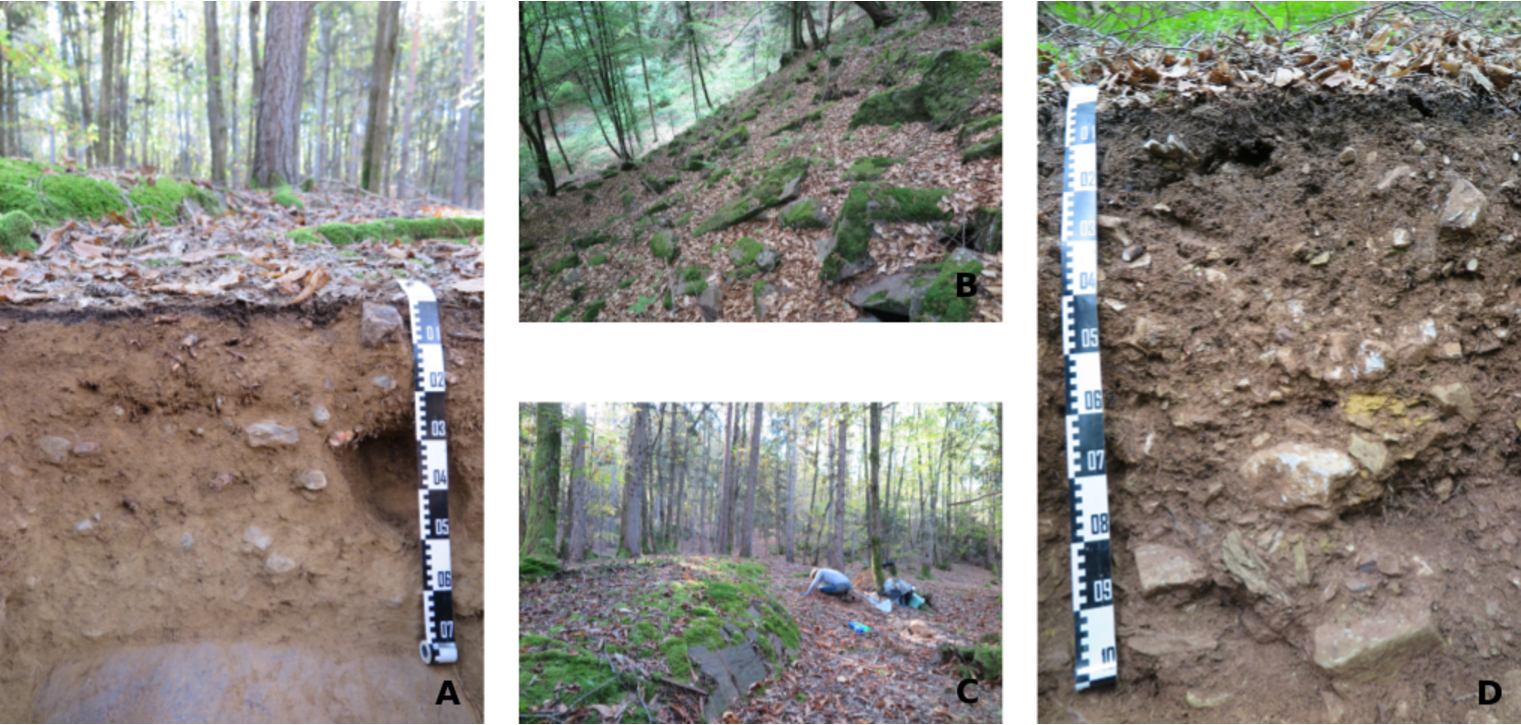
\includegraphics[width=\textwidth,angle=0]{soils_red.pdf}
\caption{A) Soil profile 39 on the SGU siliceous bedrock with parent material identified as till, representative of the typical situation of till on siliceous bedrock. B) soil profile site 39 C) Soil profile site 43 D) Soil profile 43, located above the debris cone of Andrian on the SB map unit. The yellow components are from up-slope ISR layers, while calcareous components from even higher layers can also be identified.}
\label{fig:soils}
\end{figure}
An investigation into the soil types classes of the soil profile sites located on the SGU siliceous bedrock shows that brown soils are the dominating soil type, represented by 37 of the 49 locations (75\%). The class Terrestrische Rohb\"oden, represented by the soil type Ranker, is second most common on this SGU, on which single examples of the soil types Semipodsol, Kalkbraunlehm, Farb-Substratb\"oden and Kolluvisol were also encountered. Taking into account only the soil profile sites for which the surveyors identified SB as parent material, whether or not actually located on this SGU, the soil type brown soils similarly dominates the soil type Ranker, with 13 and 6 profile sites, respectively. All of the other soil types found on the SGU on the geological map were not identified by the surveyors to have SB parent material, however one soil profile site with this parent material was attributed the soil type Grobmaterial-Rohboden. This soil type however does fit well for soils on siliceous bedrock outcrops, were only initial soil formation is possible, whereas the other soil types located on the SGU of the geological map are less plausible on SB, especially Kalkbraunlehm. In addition, the vast majority of the soil profile sites located on this SGU but identified to have a different parent material class (mostly till)  by the surveyors, also feature the soil type Braunerde, thereby decreasing the severity of misclassifying SB and TG, at least from a soil type perspective. Figure \ref{fig:soils}D shows an example of such a situation, consisting of a brown soil developed from a cover layer of till on siliceous bedrock. From this perspective, the soil type Ranker is more characteristic of the SB unit, as it is less common on TG with its characteristically more developed soils and the increased influence of  calcareous materials. Furthermore, an examination of the points were parent material classes from observation and SGU map coincide, shows a decrease in dominance of brown soils compared to Rankers, with proportions of 57 and 35 \% for both soil types, respectively. This is also well in line with the fact that SB sites are characterized by higher roughness values and situated on convex, ridge-like structures where decreased soil formation can be assumed. In conclusion, the soil types Braunerde and Ranker are characteristic of this unit, with the former representing locations were weathering and clay-reformation has led to horizon differentiation not present in the less developed Ranker soils which are found on siliceous bedrock outcrops.

\subsubsection{Till in general}
The unit till comprises lodgement and subglacial till, as well as other, undifferentiated till materials. It is found in the paleovalley as well as on flat terraces of the the Mendola-Ro\`en-Ridge.   Covering more than 25 \% of the study area, it is the most common SGU on the geological map, sharing borders with every single SGU, the longest, each with a length of at least 30~km, being those with the SGUs alluvial deposits,  siliceous bedrock and slope deposits. According to the geologic map, 109 of the soil data points are located on the SGU till, accounting for 29\% of the points. In 88 of these locations, the surveyors agreed with regard to the parent material being till, leading to a user's accuracy of 80\%. The majority of the other soil data points on this SGU were attributed the parent materials slope deposits or  mixed deposits, with some intermediary sedimentary rocks also identified as parent material. While the user's accuracy for till is the best amongst the SGUs, the producer's reliability is not comparable, as the surveyors also identified till as the parent material at 63 further locations on different SGUs. The relative majority of these locations are found on the unit siliceous bedrock, already discussed above, but a large number of soil profiles with this parent material are also located on the units calcareous sedimentary rock and slope debris. Furthermore, till was identified as the parent material of soils on the units SSR, MxD, MrD, GLD, DC, CBD and AD. An important takeaway point from these results is that while, at least for this study area, the SGU unit till is a good indicator for where to reliably encounter soils evolved from till, it is of great importance to expect this  parent material also on various other SGUs.

 A topographic comparison of those points with till as parent material located on the SGU till with points with the same parent material but on different SGUs (Table x), shows that the misclassified, latter group is characterized by a higher roughness (mean TRI of 25 compared to 13 for the correctly classified group) and steeper slope (mean value of 21 compared to 12$^{\circ}$). Regarding confusion with the soil parent material unit calcareous sedimentary rock, data mining the terrain parameters of the relevant soil profile sites again highlights the role of the parameter TRI, in this case dominantly at a window size of 50~m, in topographically separating the unit till from other parent material units. CSR profile sites are characterised by TRI values in the upper quartile of the values characteristically displayed by TG profile sites. Of the local terrain parameters, slope, together with minimal curvature, performs well in separating the points of both groups, but not as clearly as it separates both units on the geological map, as TG profile points in the study area can be found at slope values higher than indicated in the geological map. To characterise the difference of the TG sites with slope deposits, the TRI with a window size in the range of 100~m performs best of all local, regional and roughness-related terrain parameters in the forward stepwise feature selection. Similar to the situation with CSR, slope is the best performing local terrain parameter, but as before, the separation is clearer on the geological map, signifying that till can be found at steeper angles than   expected from the geological map. Till as the parent material of soil profiles on the surficial geological map units CBD, DC and GLD is not as common as for the above discussed units and additionally these units do not have as many overall members, nevertheless some interesting observations can be derived from the random forest-based investigation. For instance when compared with till, debris cones, which have a considerably uniform topography at the analysed grid cell size of 2.5~m, are characterised by lower local roughness (VR with ws = 50~m or TRI with ws=7.5~m) and a low landform diversity as represented by a high mean patch size of landforms calculated at a lookup distance of 7.5~m and a flatness threshold of 10$^{\circ}$. The profile site topography of the unit coarse blocky debris, on the other hand, is distinguishable from till by a higher TRI (ws=125m) as well as steeper slope. Other aspects that may account for the high number of till parent material sites on units other than till have been discussed in the siliceous bedrock section.
 
 Typical for the study area, and especially characteristic of the till parent material unit, brown soils dominate the soil types of the profile sites on the corresponding  map unit with 59\%, but even more so when considering only the sites for which the surveyors identified till as parent material (70\% of 151 profile sites). This proportion is comparable to that of brown soils for the data subset for which till is indicated as parent material by both the surveyors and the geological map. While brown soils also dominate on SB, the variety of subtypes on till is greater. While SB shows mainly typical brown soils and some with signs of beginning podzolisation, these subtypes are accompanied on till by brown soils containing calcareous components as well as brown soils characterised by higher clay contents, a strong influence of the clay on horizon differentiation (soil type Textur-Substratboden), and also vertical translocation of these particles (soil type Parabraunerde, which developes only on this parent material in the study area). The latter soil types and subtypes are common on till parent material, especially when developed on sub-glacial or lodgement till.  The presence of soils of the class of Umgelagerte B\"oden, i.e. soils that have been rearranged vertically or horizontally either directly or indirectly by human influence, can be accounted for by the fact that most vineyards or apple orchards are located on this unit. Of the class of less developed soils with only an organic horizon (Terrestrische Humusb\"oden), accounting for 13\% of the soils with the parent material till, the majority is influenced by the calcareous components of the till, separating these soils from those on SB. The role played by the calcareous till material, brought into the till mainly locally from the slope of the Mendola-Ro\`en-Ridge, is also highlighted by the presence of soils of the class Kalklehme. In summary, the soils of the SGU till are characterised by well developed soils, often with calcareous properties. This is will in line with the topography of this unit, distinguished by low roughness and gentle slopes.


\subsubsection{Slope debris}
\label{section:results_SD}
Slope debris, as a SGU of the geologic map, occupies 10\% of the study area. Its by far longest border is shared with the unit siliceous bedrock, other important borders are with the units till, calcareous sedimentary rock and debris cones, the first three units greatly influencing the distribution of components in the slope debris units. When comparing the parent material of soil profile sites with the SGUs , the slope debris unit has slightly better user's accuracy than producer's reliability, as surveyors established slope debris as the parent material of 55 of the 84 profile points on this SGU, but also for 69 soil data points on other SGUs. Similar to the SGU siliceous bedrock, the most confusion regarding parent material on the SGU slope debris occured with the unit till, which was identified at 15 soil profiles. As is the case with the SB unit, some of this confusion may be attributed to thin layers or punctual deposits of till. Considering slope debris, another important aspect is that the debris in question may very well be composed of till material that has been transported gravitationally. The same explanations may hold for other parent materials which were identified on the slope debris unit, especially for the bedrock units SB, ISR and  CSR. While some isolated outcrops are possible, the most likely cause is that the constituents of the slope debris are so dominated by transported material of one of these bedrock classes, that the surveyors determine this unit as the parent material of the examined soil profile. On the other hand, misclassification between the units coarse blocky debris and slope deposits can be attributed to the fuzzy border between these units, ultimately linked to the grain size distribution, and the subjective interpretation thereof, especially during field survey. 
Contrary to most other SGUs (with the exception of CBD, LD and MxD), this unit itself does not provide information regarding the mineralogy of its component, which can only partially be derived through  interpretation  of its location in the catchment and the uphill geologic situation. Consequently, this unit  is much better described by its topography than its material, as the latter may be highly diverse. 

Those profile sites for which the geological map correctly proposes slope debris as the soil parent material differ from the slope deposit points on other SGUs mainly by higher slope heights and also higher slope angles, that is the geological map tends to under-represent slope debris situations in lower regions of the catchments and at less steep positions. 20 of the 122 soil profiles with slope debris as parent material are located on debris cones according to the geological map, which are good examples of the mentioned situation. This is presumably closely related to the furrowed and disturbed character of debris cones in the southern half of the study area, where the situation may not present itself clearly during field survey. Additionally, the material composition as well as its origin is basically the same for slope debris and debris cones in this area. Topographically, roughness measures do well in seperating the slope debris points from the debris cones points of the field survey data set. Slope debris  is characterised by higher vectorruggedness (ws=52.5~m) values, which are very low for debris cones. Slope angles also differ considerably, implying that the surveyors tend to annotate slope debris if the topography does not show the low roughness and slope values characteristic of debris cones. This difference of roughness and slope with regard to the conceptual difference of slope debris and debris cones is also apparent when comparing the topography of both units as delineated by the geological map, however the difference is more distinct in this case. Similarily, calcareous sedimentary rock as parent material seems connected to roughness values slightly higher than those present for the average slope debris site, a relationship which is again more pronounced in the geological map. Consequently, it is in these transitional zones were the misclassification occurs. This topographical proximity of the units is of course  reinforced by the fuzziness of distinguishing between the two parent material as such. As is the case with siliceous bedrock and slope debris, the border between the  source material, in this case the calcareous bedrock, and its derivative, the slope debris, is often not clear when considering the parent material of a soil profile. The degree of weathering of the source material certainly adds to the confusion. The  issues are comparable for the parent material units intermediate and siliceous sedimentary rock. While the gradual transition from source material, in these cases bedrock of differing mineralogical composition, to slope debris poses various issues that cannot be explained only by topography, this is even more the case when considering the possibility of confusion between slope debris and coarse blocky debris, the distinction between which raises a number of questions with regard to the objectivity of  estimating block or grain size of soil profile parent material. Misclassification between the units slope debris and mixed deposits are also predominantly a question of definition and the explanatory power of topography is very limited.

Given its confounding nature, due to its dynamic topography and  great variability of components, this unit shows a high diversity of soil types, encompassed only by the parent material till due to its variety of anthrosols and well developed soils.  With regard to soil type classes, the class incorporating soils with only organic layers on top of parent material (Terrestrische Humusb\"oden) stands out, both with respect to the soil profiles on the map unit (70\%) as well as those for which surveyors specified the parent material slope debris (64\%). While both of these approaches of analysing the distribution of soil classes have brown soils (25 and 15\%, respectively) as the most important secondary soil class, the main differences are the classes Kalklehme and Umgelagerte Böden, of which the latter is found only from the viewpoint of the soil profile descriptions. The presence of multiple soil profiles of the Kalklehm class shows that soil surveyors are more likely to identify slope debris as the parent material also for locations which are more favourable to soil formation than the areas indicated as this SGU on the geologic map. This is indeed consistent with the topographic analysis of the profile points. Similarily, these transitional locations between steepers slope and flatter regions are also indicative of the confusion between slope debris and debris cones, exemplified by the relatively large proportion (12\%) of Rigosols, which also highlights that soil surveyors tend to emphasize the components, in this case slope debris, instead of the geomorphological form as presented by debris cones. In summary, soils with only organic horizons are the most common representatives of soils on this parent material, with those related to calcareous parent material (Rendzina aand Kalklehm-Rendzina) more prevalent than their siliceous counterparts, especially when considering only those soil profile locations for which surveyors identifed slope debris. Nevertheless, soils developed from slope debris can show signs of advanced soil formation in less sloping, smoother topography, for instance in bordering debris cones or other deposits. 
\subsubsection{Calcareous sedimentary rock}
The calcareous sedimentary rocks in the study area are predominantly  responsible for the steep walls of the upper elevations of the  Mendola-Ro\`en-Ridge (Dolomite and limestone), but also represent some thin layers in lower parts of that slope, interchanging with intermediate and siliceous sedimentary rock layers. Despite covering only 8.4\% of the area, it has long borders due to its layers that span from north to south of the study area. Slope debris units often occupy locations downslope of the CSR units, accounting for the long  border length of 40~km with this unit. The fuzzy transition from weathered bedrock to slope debris is a major issue also for this SGU. The confusion matrix representing the comparison of the parent material as indicated by the geologic map and the parent material identified in field survey (Table \ref{kartiergegenkarte}) shows that, consequently, this is the unit responsible for the most misclassification, contributing to the very low user's accuracy of this SGU. Additionally, due to its intermittent layering with ISR, it is not surprising that this unit was found to be the parent material for 7 investigated soil profiles in the calcareous sedimentary rock unit. The producer's reliability is slightly better, however, all in all only five of the soil profiles were attributed the parent material unit calcareous sedimentary rock, of which two were in fact situated on the SGU slope debris. This again accentuates the problem with differentiating these two units when adjacent, as one is often the result of weathering, and gravitational transport, of the other unit. Similarily to the other bedrock units in the study area, till was reported also in this unit as the soil parent material at 12 sites, accounting for a third of the soil profile locations on this SGU and highlighting the necessity to expect thin layers of till in areas mapped as bedrock. Due to the small number of soil profile points actually identified as haveing CSR as parent material, the random forest classification approach of identifying important terrain parameter differences between the correctly classified points and those on other units is not very meaningful. Topographical separation from intermediate sedimentary rock, a major cause of misclassification, is also not very adequate, as the most important parameter in this case is slope height. This is to be expected, since the main difference is the vertical position in the overall geological structure of the study area, a difference which is however diminished by the above mentioned intermittent layering and gravitational movement down-slope, in addition to the above discussed problem regarding the definition of slope debris versus weathered bedrock.

The Rendzina is the typical proponent of soil types on calcareous sedimentary rock, as exemplifizd by the two soil profile sites for which both the geologic map and the surveyors indicated this unit as the soil's parent material. The situation described in the topographical description of the units leads to a high number of soil profiles along with a variety of different soil types. These include soils were soil formation processes have lead to horizon differentiation such as Braunerde and Kalklehme, nevertheless the class Terrestrische Humusb\"oden consitutes the majority. However considering only the soil profiles sites that qualify for CSR parent material from the surveyor's point of view, this is the only class, represented by the soil types Rendzina  and Kalklehm-Rendzina. Given the topographic situation and the complex geologic setting, it is necessary to assume the possibility of soils with signs of increased pedogenetic developement on this map unit, however a different parent material such as till or slope debris of varying composition must be considered for any of these soiltypes. 

\subsubsection{Debris cones}
The unit debris cones are located west of the center of the paleavalley, between the slope debris of the Mendola-Ro\`en-Ridge slope in the west, which are often the source area of these deposits, and the till deposited in the paleovalley in the east. Other units with which long borders exist are mixed, colluvial, and alluvial deposits. The number of profile sites is comparably small with 36 profile sites, considering that the unit occupies almost 13\% of the study area. A reason is that a large part of the debris cones are covered by settlements.  Although the soil surveyors noted debris cones as parent material for only five soil profile sites, it must be considered that 20 of the misclassified parent materials on the debris cones unit were identified as slope debris. Given the long mutual border and the fact that the source of the debris cones material is mainly the slope debris and the calcareous bedrock units which themselves are the origin of the slope debris, this misclassification may seem acceptable. In fact, it rather points out a difference in the point of view of the soil and the geologic surveyors, where the first are interested in the material and the latter more in the landform presented by the debris cones unit. The remaining misclassifications are all with units that border this SGU, or, in the case of intermediate sedimentary rock, are located in the source region of the the debris cones.

The topographic issues regarding the confusion with other parent materials such as AD, SD, TG have been discussed in the unit-specific subsections, highlighting this units landscape position as the main distinguishing characteristic.

As discussed, compared to the number of soil pit locations for which the surveyors identified the parent material class debris cones, the number of sites located on this unit of the geological map is much higher, which also leads to a greater soil type variability, especially at subtype level. While surveyors identified this unit only once for more developed soil types such as Braunerde or Kalklehme, they constitute 42\% of the sites indicated on the map. Given the strong anthropogenic influence on debris cones, a large proportion of the profiles have experienced vertical anthropogenic rearrangement, in an effort to enhance the general conditions for viticulture. Soils with only organic layers can also be found in areas with less intensive anthropogenic influence, though more commonly on areas where only the geologic map indicates debris cones, whereas the surveyors more commonly classified the parent material as slope debris, highlighting the issue of defining the difference, as discussed in section~\ref{section:results_SD}.

\subsubsection{Intermediate sedimentary rock and siliceous sedimentary rock}
The units intermediate and siliceous sedimentary rock are situated in the slope of the Mendola-Ro\`en-Ridge and are characterised by  more or less thin layers, often intermittent with layers of calcareous sedimentary rock, and only a limited amount of outcrops. Another common characteristic is that none of the soil profile points for which the surveyors identified one of these units as the soil's parent material is actually situated on the corresponding geological map unit. The parent material of all three soil profile sites on ISR was classified as slope deposits, which is understandable considering the issues discussed in the previous sections regarding slope debris and weathered bedrock. As further evidence of this issue, ISR was detected as the parent material of four soil profiles on the map unit slope debris. Additionally, intermediate sedimentary rock was identified as the parent material of 7 soils on the CSR map unit and two on the SSR unit. There is of course no question that the layers are correctly located on the geological map with regard to the underlying geological structure of the study area, these soil profile sites rather highlight the possibility of finding any or all of the materials of these intermittent layers on these units as well as any potential down-slope slope debris units due to the prevailing geomorphological dynamics in the study area. Gravitational transportation leads  to these materials serving as soil parent material not where the layer is indicated on the geological map, but in fact down-slope of these layers. Additionally, these materials are seldom found as homogeneous units due to mixing and multi-layering caused by gravitational transport. For these and other reasons discussed in the CSR section, topographical separation is limited for these units. 

As the situation described above does not seem to favour soil formation processes to take place in a constant manner, it is surprising that while two out of the three soils on the geological map unit belong to the class Terrestrische Humusb\"oden, the majority of the soil profile sites specified as having ISR or SSR as parent material are of the classes Braunerde or Kalklehme, i.e. soils with A and B horizons. More expected is the presence of colluvisols on the SSR units (both on the map and regarding field survey).  In summary, it appears that in such a dynamic environment as on the SGUs ISR, SSR and slope debris, soil surveyors tend to notate slope debris as the parent material of less developed soil such as those of the Terrestrische Humusb\"oden class, while placing more emphasis on the the mineralogical properties of the components when describing soils that experienced more pedogenetic processes. Nevertheless, this analysis implies that soils developed from any of these intermittent layers are more likely to be encountered in down-slope slope debris units, especially for ISR. Regardless of the present dynamics, more evolved soils are possible but may present very heterogenous parent material due to multi-layering. Figure~\ref{fig:soils}D shows an example of such a profile site in steep topography with a typical slope debris parent material mixture containing ISR material, which has however been deposited on a SB unit located downslope of the layers.




\subsubsection{Colluvial, mixed, and landslide deposits}
All three of these SGUs are characterised as material that has been transported down-slope by various processes. Regarding colluvial deposits, the surveyors indeed identified this parent material unit for three of the five profile sites on this map unit. The parent material of the remain two sites was mapped as ISR and SD. While the latter can be attributed to the similarity of the material and the uncertainty of the definition of the difference between slope deposits and colluvial deposits, the former can also indicate that the soil surveyor may value the information with regard to the mineralogy of greater importance to explaining a soil profile  than the information regarding the morphydynamic history of the material. The definition of mixed deposits as deposits from debris flows, torrents and avalanches is similarly dominated by the means of transportation rather than the material components. Interestingly, none of the soil profiles located on this map unit were linked to this parent material by the surveyors, but five of the profiles on till were. With regards to soil parent material, an important issue is whether this material is in fact constituted of the same material as till and has been simply transported by one the mentioned processes. The parent material of the majority of the soil profiles on the  MxD unit of the geological map were identified as slope deposits, highlighting the definitional proximity of these units, at least concerning the view of surveyors focussing on soil. Compared to these two units, the issue regarding landslide depositions is different one. This unit was never used by surveyors to describe the parent material of a soil profile site. Of the three data points on this map unit, the surveyors explicitly chose the parent material siliceous bedrock of two locations, which is in fact the material of the landslide body in the study area. Coarse blocky debris was also used at one soil profile site, which well describes the  structure of the material involved. This example provides insight into how the different emphasis and focus of soil and geologic surveyors influences their classification, each highlighting a different aspect of the same unit.

Topographically, these three units are not easy to differentiate, especially with regard to the unit slope debris, which is very close with regard to both definition as well as morphometry and discussed in the slope debris subsection.


The soil types of the three soil profile sites with parent material which both geological map and surveyors identify as colluvial deposits, are of the classes Umgelagerte B\"oden and Brown soils and are representative of both the map unit and the soils as attributed by the surveyors, although the latter also link this parent material unit to a less developed soil like Ranker. In general, the colluvial deposits are characterised, or understood, as the accumulation of eroded slope material, which can also be A-horizon material  for instance from agricultural lands. Consequently, disturbed soils but also better developed soils on older accumulations are  conceivable examples of soils on CD. 
Given the similar genesis of mixed deposits, the soil classes distributed amonst gthe soil profiles with this parent material are comparable, despite some of the points being located on TG according to geologic map. But as this parent material can actually be till or calcareous sediments transported from up-slope locations, the soils types Braunernde and Kalklehme are good fits and show that confusion between the units does not lead to severe misclassifications, at least from a soil surveyor's point of view.    
As discussed in the topography section, the landslide mass in the study area is composed of sliceous bedrock, with the soil types Ranker und Braunerde being typical and as anticipated for soil developed from such parent material. 

\subsubsection{Glacio-lacustrine deposits, ice-marginal sediments and mire deposits}
Even when taking into account that only seven soil profile sites are located on this map unit, the geological map has a relatively good user's accuracy for the soil parent material unit glacio-lacustrine deposits. It comprises both glacio-lacustrine and lacustrine deposits which are conentrated at the northern border of the paleovalley. The producer's reliability is below 0.5, as surveyors indicated this parent material also for soil profile sites on the SGUs alluvial deposits,  mire deposits, siliceous bedrock and till. Confusion with the first two SGUs seems acceptable due to the common fluviatile or hydromorphic history, although the other misclassifications do indicate the possibilty of local glacio-lacustrine deposits as the parent material on these units. The topographical analysis of those points on other SGUs but with GLD as the surveyed parent material hints that these are located in regions where landform diversity is partly dominated by a single class at meso scale (ws=50~m), indicating a smoother surface than for the GLD map unit, as well as being characterised by a more pronounced negative minimal curvature suggesting concave topography. The random forest-based investigation into the topographical difference between soil profile points with SB and with GLD as parent material characterize the latter with lower roughness values  (TRI and vectorruggedness at window sizes between 100-130~m), indicating similar regions on SB as possible GLD areas. Regarding soil type, investigations from both viewpoints, i.e. from the geological map and the soil profile data, show the soils on this unit as belonging to either the soil type Braunerde or Rigolboden, the latter representing agriculturally used land. Due to the lack of profile points in mire deposits, GLD is the only SGU on which surveyors mapped a hydromorphic soil type, in this case Pseudogley.

Ice-marginal sediments are closely associated with till units and are mostly located in close proximity, consequently shareing  long borders. Given their often thin, elongated form and the fact that they cover only 0.2\% of the study area, only one soil profile site is located on this SGU on the geologic map, of which the parent material however is classified as alluvial deposits. This situation again highlights the problem fuzzy definitions that may overlap between closely related parent material units. Similarily, it may not be as important to the soil surveyors that the gravelly parent material is of ice-marginal origin, compared to alluvial, as it is to the geologic surveyor specialized on the quarternary. 
Similarily, on the SGU mire deposits the surveyors identified the soil parent material glacio-lacustrine deposits twice and till once, with the only soil profile with mire deposits as parent material being an anthrosol (filled mire deposit) located on the SGU till. The influence of stagnant water on both GLD and MrD can help understand the confusion between both units, and local mire deposits due to reduced permeability on clay-rich sub-glacial till is also rather likely. Given these local phenomena as well as the small number of sample profile sites, the topographical seperation of the units IMS and MrD provides little relevant information, as does an analysis of soil type distribution.
 
\subsection{Random forest classification of parent material based on geologic map data and topography}
The result of the feature selection procedure for predicting parent material classes was that, without exception, the SGU information was chosen first in every single feature selection run. This is important as it also contains information on the confusion between certain classes implicitly in the sample point data. Contrary to when investigating which terrain parameters best highlight the differences between two specific parent material units, local and regional terrain parameters, including relative elevations, were not identified as important predictor variables. Instead, the roughness-related measures dominated the selection process, even with the parameter set including all available terrain parameters, resulting in the choice of two of these measures and the SGU-information. The addition of further explanatory variables was not seen as an  improvement with regard to both the model performance as well as its interpretability after evaluating some possibile expanded models both with visual inspection of the results as well as the one-standard error rule \citep{James2013}.  The reason for the decreased importance of regional, but also local, terrain parameters is that this information is already implicitly accounted for by the geologic map, as the various SGU classes are closely linked to certain relative elevations, especially the vertical distance to channel base level, due to overall geologic structure of the study area. Additionally, at least to a certain degree, some units like till, slope debris or alluvial deposits also provide implicit information regarding slope angles. Furthermore, a certain amount of slope information is also included in the TRI, which increases with slope as well with increasing roughness. The vector ruggedness measure well compliments the TRI and the SGU as it provides information on surface roughness independent of the slope gradient. Figure~\ref{fig:SGUandmodel} shows the original SGU map (A) as well as the parent material map based on SGUs, TRI and vector ruggedness (B).
 \begin{figure}[ht!]
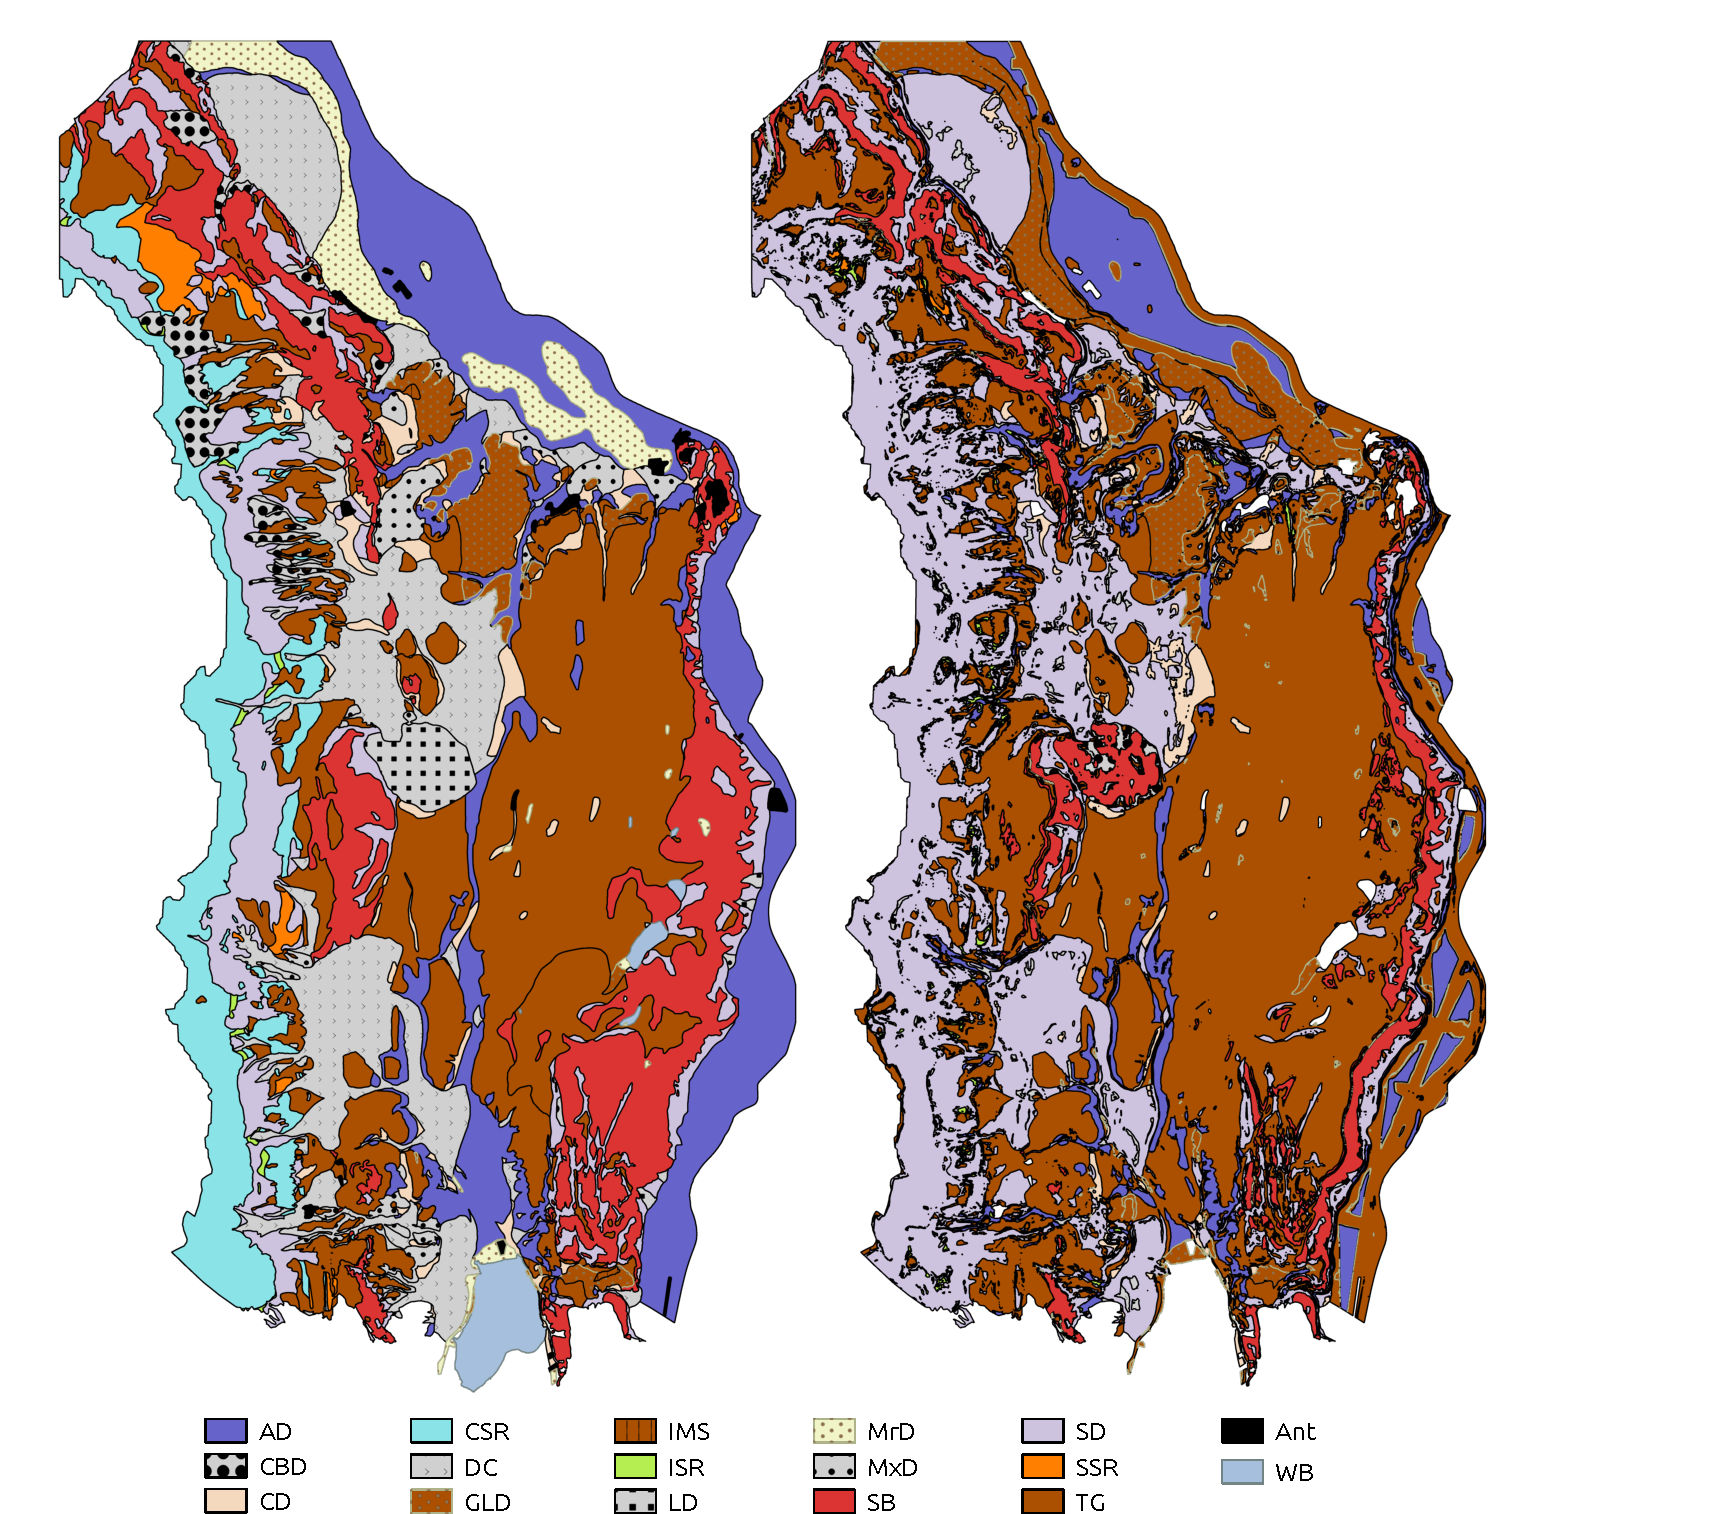
\includegraphics[width=\textwidth]{SGUandmodel.pdf}
\caption{Original reclassified SGUs (A) and random forest-based parent material map modified based on vectorruggedness and TRI (B) and parent material map with only till modeled (C) }
\label{fig:SGUandmodel}
\end{figure}
This modeled parent material map leads to an overall accuracy of approx. 90\%, however the out-of-bag correct classification rate= only 65\%, implying quite substantial overfitting. Consequently, the predicted map must be evaluated with caution. A comparison of the resulting SGU map, adjusted only by adding two roughness parameters, with the original SGU map, reveals a considerable areal increase of the TG unit. This is perfectly understandable given the low producer's reliability revealed in Table~\ref{kartiergegenkarte} by the high number of soil profile sites located on different SGUs but with TG as the surveyed parent material class.  The most obvious errors linked to this unit are the roads as well as the mire deposits surrounding the large debris cone in the north, which are modelled as TG. Similarly conspicuous is the fact that the areas originally covered by the SGUs debris cones and mixed deposits now seem to be covered by the slope debris unit, which seems contrary to the good prediction results of these units. Detailed investigation into this issue shows that overfitting ocurred in these cases, with very small, local DC and MxD polygons leading to the false impression of correct classification. On the other hand, the severity of this misleading results may appear less grave when  considering the similarity of these three units. Given that they all represent material that has been transported down-slope by various processes and that their composition may in fact be the same in many cases, this misclassification may seem acceptable if one keeps in mind the information provided by the original map with regard to the geomorphological history of these units. Small units like CSR, ISR and SSR are taken over by slope debris and or till in a similar manner. An interesting unit in the predicted map is the former landslide deposit in the center of the study area. As the surveyors put more emphasis on describing the deposited material itself than its geomorphological history, the unit is now modelled as siliceous bedrock with coarse blocky debris, which well represents the view of the soil surveyors.  Another insightful aspect of the predicted parent materials are new, additional polygons which suggest small glacio-lacustrine deposits inside the largest till unit east of the Mitterberg. Based on the experience from previous field work in this area, the authors deem this assumption worthy of future investigation.

After considering and evaluating the issue that arise with regard to the individual SGU as well as from modeling parent material for the study area, it was concluded that while the parent material is helpful in giving insights into issues that arise when using geologic maps and topography as a proxy for parentmaterial, to much of the information provided by the original SGU map is lost in the new, predicted parent material map. The under-representation of the class till, however, which had been identified as the main single issue when applying the geologic map for soil survey, seems to have dealt with appropriately by the random-forest classifier. Hence, a new approach was chosen by modelling only the till class and then overlaying this information onto the original SGU map. The forward step-wise feature selection procedure for the units till vs. not-till again chose one TRI and one VR map as model input features, but with slightly differnt window sizes (100~m and 102.5~m, respectively) than for the parent material model. This approach combines the models good performance with regard to modeling the often thin till layer, while retaining most of the information from the geologic map (Figure \ref{fig:SGUandmodel}C), which can help in understanding the composition of slope debris and other transported materials. Compared to the original confusion matrix (Table~\ref{kartiergegenkarte}), the overall correct classification rate is improved form 49\% to 65\% with this approach.

\subsubsection{Discussion of accuracy} 
As \cite{Olofsson2013} point out: uncertainty in remote sensing applications, but also in general, can be related to geolocation and interpreter  variability. In this study...

-multiple interpreters, but not on same profiles, what about powell 2004 and their five interpretators  

-Wickham 2013: constant communication in order to discuss and documen difficult cases is important

- in future: response protocols!
\subsection{Differences between geologic survey and parent material from profile site descriptions} 
\subsection{General difficulties} 
\begin{itemize}
\item confusion at categorical transitions
\item analyst biases (Foody 2010)
\item \cite{Olofsson2013} state that with regard to reference labeling, in this case the parent material, difficult case need be noted for future reference and consensus development
\end{itemize}
\subsubsection{Differences with regard to mapping purpose}
Between the two different frameworks of mapping, geology on the one hand and soil on the other, it is important to acknowledge the main focus of attention of each branch of research. There may exist a difference with regard to how pronounced a certain feature or characteristic must be in order to considered for mapping. \cite{Miller2015a} note that the resulting maps of the two sciences try to communicate different aspects. While geology refers to geologic materials and general landform regions, soil science is concerned more with soil properties with regard to land use and management decisions.

A typical example is the unit landslide debris, which seems only of interest to the mappers with focus on geology, whereas the soil surveyor...

Regarding glacial deposits, the soil or forestry surveyors seldom differentiated between lodgement till and other glacial deposits, only when an decisively higher clay content was determined. On the other hand, the chemical properties, especially with regard to acidic properties of the tillic material are of much more interest to the soil surveyors who further differentiate till with regard to this aspect. The geologic map on the other hand also contains information with regard to the age and the geologic system(synthem) to which certain moraines belong, whereas this is only of interest to the soil surveyor if it features additional information with regard to the mineralogic content of the different constituents of the moraine.

Geologist only map regolith cover layers thicker than approximately 1~m.

What is more important for soil mapping, the transportational history of material or information regarding its composition?

\subsubsection{Nomenclatural differences and overlaping classes}
Congalton 

\subsection{Pedologic interpretation of terrain parameters that best seperate the geological units}
Do the points surveyed as moraine have different terrain parameters from those mapped as moraine on the geologic map.
\subsection{Distribution of soil types with regard to geologic unit as well as parent material unit}

\subsection{Influence of the Alpine environment on interpretability of geologic units as parent material units}
\cite{Heung2014} note that while traditional geologic maps focusing on bed rock are a valuable input for DSM when the residual materials form the soil parent material, but less so in areas distinguished by glaciation and hgih geomorphodynamics. Similarily, in their comparison of surficial geology maps derived from Soil Survey maps on the one hand and the Geologic Survey on the other, \cite{Miller2015a} point out that the level of aggreement was lower for areas with complicated geologic histories.

\subsubsection{High relief areas and multilayering}
Are there thresholds regarding terrain parameters?
\subsubsection{thin cover layers of till - an essential new parentmaterial unit?}
Why is important to differentiate till and slope debris? While there may exist situations were the slope debris is composed of till material, the general difference is that soils from slope debris can be understood with knowledge of local geology and that they may not be so different from soils higher up in the catchment that evolved from bedrock, whereas till can consist of chmically very different components.
Till can be found at steeper slopes than expected, is this due to lateral consolidation of tillic material by glaciers in thses U-shaped valleys?
\subsubsection{Is the morphodynamic background of deposits a necessary distinctive attribute from a pedological point of view?}
In the study are, mixed deposits from mass movement and torrents have the same components as till or hillside debris, which themselves are often the same...

\subsection{Terrain parameters - issues and results}
\begin{itemize}
\item the landform diversites are all heavily correlated and have the same meaning in the end.
\item beware of the different class sizes when using random forest and boxplots to investigate differences
\item In general local terrain parameters and regional terrain parameters are only important if the parent material map does not apply the information already implicitly provided in the new detailed geological map.
\end{itemize}

\section{Conclusion}
We propose that future surveys focus increasingly on these units with greater uncertainty with regard to soil parent material to strengthen understanding of the pedologic relevance of these units. By performing a GTC prior to future detailed field soil surveys, the surveyor can make best use of available information and concentrate the time and money consuming task of field work, involving soil pits and auguring, on units identified as highly variable and uncertain regarding soils. This information can be additionally helpful for devising future sampling procedures and also for consideration when attempting to regionalise point information.

\section*{Acknowledgements} This research was performed within the project 'Terrain Classification of ALS Data to support Digital Soil Mapping', funded by the Autonomous Province Bolzano -- South Tyrol (15/40.3).

\section*{additional tables}
\begin{table}[ht]
\centering
\tabcolsep=0.06cm
\small
\begin{tabular}{ccccccccccccccc}
  \hline
 & CBD & CD & CSR & DC & GLD & IMS & ISR & LD  & MrD & MxD & SB & SD & SSR & TG \\ 
  \hline
AD & 0.2 & 21.1 & 0.0 & 23.6 & 14.8 & 2.5 & 0.0 & 1.2  & 22.2 & 10.9 & 5.7 & 12.7 & 0.2 & 45.2 \\ 
  CBD &  & 0.5 & 6.1 & 8.5 & 0.0 & 0.0 & 1.1 & 0.9  & 0.5 & 1.5 & 10.1 & 9.7 & 0.9 & 9.1 \\ 
  CD &  &  & 1.3 & 17.6 & 10.7 & 2.8 & 0.0 & 0.6  & 0.7 & 10.0 & 5.8 & 4.0 & 0.0 & 31.1\\ 
  CSR &  &  &  & 11.8 & 0.0 & 0.0 & 5.5 & 0.8  & 0.0 & 1.3 & 0.6 & 40.7 & 5.0 & 23.1 \\ 
  DC &  &  &  &  & 2.5 & 0.6 & 0.7 & 2.4  & 5.9 & 17.4 & 9.3 & 25.6 & 1.6 & 40.6 \\ 
  GLD &  &  &  &  &  & 2.2 & 0.0 & 0.2  & 0.8 & 3.4 & 0.4 & 0.5 & 0.0 & 7 \\ 
  IMS &  &  &  &  &  &  & 0.0 & 0.0  & 0.0 & 0.6 & 0.7 & 0.4 & 0.0 & 1.1 \\ 
  ISR &  &  &  &  &  &  &  & 0.2 & 0.0 & 0.0 & 0.0 & 4.3 & 0.0 & 0.4 \\ 
  LD &  &  &  &  &  &  &  &   & 0.0 & 0.1 & 1.4 & 3.7 & 0.5 & 4.2 \\ 
  MrD  &  &  &  &  &  &  &  &  &  & 0.2 & 1.2 & 0.6 & 0.0 & 1.9 \\ 
  MxD  &  &  &  &  &  &  &  &  &  &  & 2.7 & 2.7 & 0.1 & 19.5 \\ 
  SB  &  &  &  &  &  &  &  &  &  &  &  & 109.3 & 4.4 & 67.4\\ 
  SD  &  &  &  &  &  &  &  &  &  &  &  &  & 8.3 & 50.4 \\ 
  SSR  &  &  &  &  &  &  &  &  &  &  &  &  &  & 5.5 \\ 
   \hline
\end{tabular}
\caption{Length in kilometers of the borders of adjacent SGUs} 
\label{table:borderlength}
\end{table}
\section*{References}
\bibliography{P2.bib}

\end{document}